\documentclass[border=4pt]{standalone}
\usepackage{tikz}
\usepackage{pgfplots}
\pgfplotsset{compat=1.18}
\usetikzlibrary{shapes.geometric,arrows.meta,positioning,calc,fit,decorations.pathreplacing,backgrounds}
\definecolor{boxblue}{RGB}{225,238,252}
\definecolor{boxgreen}{RGB}{225,247,231}
\definecolor{boxorange}{RGB}{253,236,216}
\definecolor{boxgray}{RGB}{237,237,237}
\definecolor{boxred}{RGB}{253,226,226}
\begin{document}
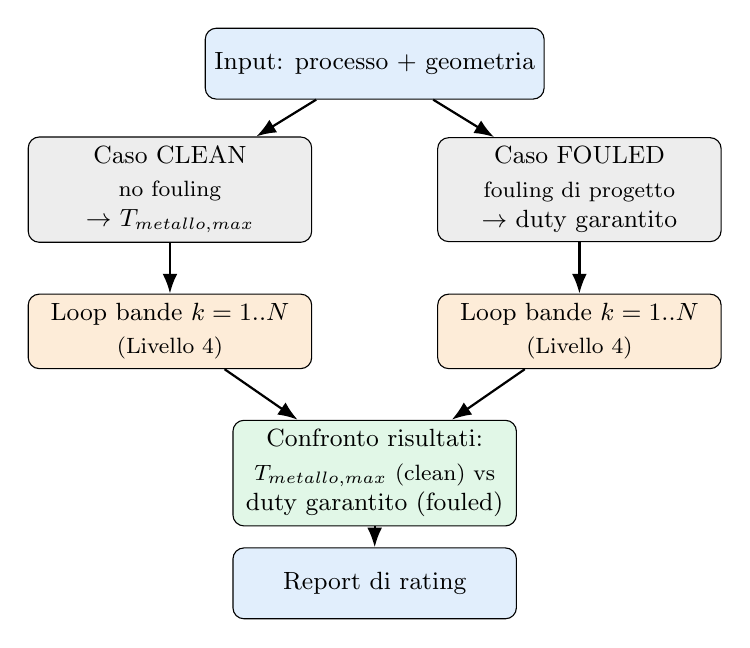
\begin{tikzpicture}[
  box/.style={draw, rectangle, rounded corners, minimum height=0.9cm, minimum width=3.6cm, align=center, font=\small},
  dec/.style={draw, diamond, aspect=2.2, align=center, font=\small, inner sep=2pt},
  arr/.style={-{Latex[length=2.5mm]}, thick}
]
\node[box, fill=boxblue] (start) at (0,0) {Input: processo + geometria};
\node[box, fill=boxgray] (case1) at (-2.6,-1.6) {Caso CLEAN\\[1pt]\footnotesize no fouling\\ $\rightarrow$ $T_{metallo,max}$};
\node[box, fill=boxgray] (case2) at (2.6,-1.6) {Caso FOULED\\[1pt]\footnotesize fouling di progetto\\ $\rightarrow$ duty garantito};

\node[box, fill=boxorange] (loop1) at (-2.6,-3.4) {Loop bande $k=1..N$\\[1pt]\footnotesize (Livello 4)};
\node[box, fill=boxorange] (loop2) at (2.6,-3.4) {Loop bande $k=1..N$\\[1pt]\footnotesize (Livello 4)};

\node[box, fill=boxgreen] (merge) at (0,-5.2) {Confronto risultati:\\[1pt]\footnotesize $T_{metallo,max}$ (clean) vs\\ duty garantito (fouled)};
\node[box, fill=boxblue] (report) at (0,-6.6) {Report di rating};

\draw[arr] (start) -- (case1);
\draw[arr] (start) -- (case2);
\draw[arr] (case1) -- (loop1);
\draw[arr] (case2) -- (loop2);
\draw[arr] (loop1) -- (merge);
\draw[arr] (loop2) -- (merge);
\draw[arr] (merge) -- (report);
\end{tikzpicture}
\end{document}
